\title{On $hp$-Adaptive Solution of Complete Electrode Model Forward Problems of Electrical Impedance Tomography}
\author{} \institute{}
\tocauthor{\underline{Harri Hakula}, Nuutti Hyvnen, Tomi Tuominen}

\begin{center}

\textbf{\Large On $hp$-Adaptive Solution of Complete Electrode Model Forward Problems of Electrical Impedance Tomography}\\
\vspace{10mm}
{\large \underline{Harri Hakula}, Nuutti Hyvnen, Tomi Tuominen}\\
Aalto University School of Science and Technology\\
Institute of Mathematics\\
Otakaari 1 \\
FIN-00076 Aalto\\
{\tt Harri.Hakula@tkk.fi, nhyvonen@math.tkk.fi, tatuomin@math.tkk.fi}

\end{center}

\section*{Abstract}

In this paper we discuss the use of $hp$-adaptive methods of Houston \& S\"uli-type \cite{HT} within our own Mathematica implementation in Complete Electrode Model
(CEM) forward problems  of electrical impedance tomography \cite{LHH}. CEM problems are diffusion problems with Robin-type boundary conditions over parts of the boundary, the electrodes. Inside the domain there are regions, inclusions, where the diffusion or conductivity coefficient varies from the default value. The task is to simulate voltage measurements with and without inclusions on the electrodes when a given current pattern is fed through electrode pairs. Using these potentials, which can be measured in practice, reconstructions of the conductivity can be computed. For an $N$-electrode configuration with inclusions there are $N-1$ different forward problems to solve. We focus on strategies for solving this problem set accurately and efficiently.

\begin{figure}[h]
\centering
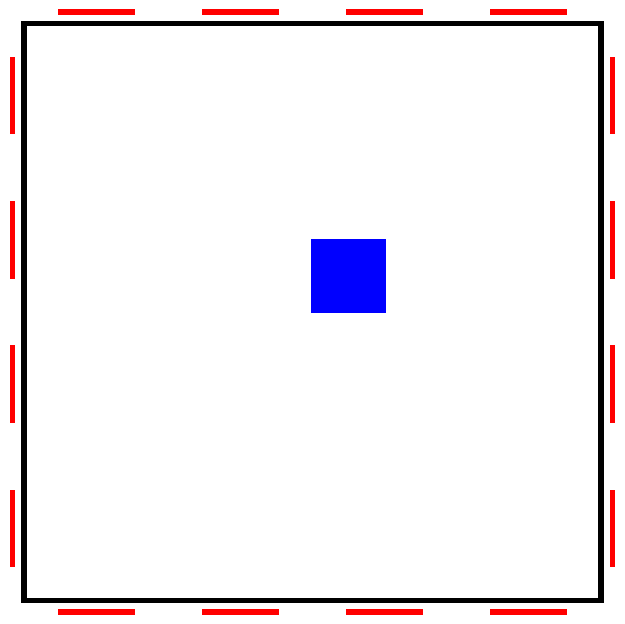
\includegraphics[width=0.15\textwidth]{./hakula/domain}\qquad
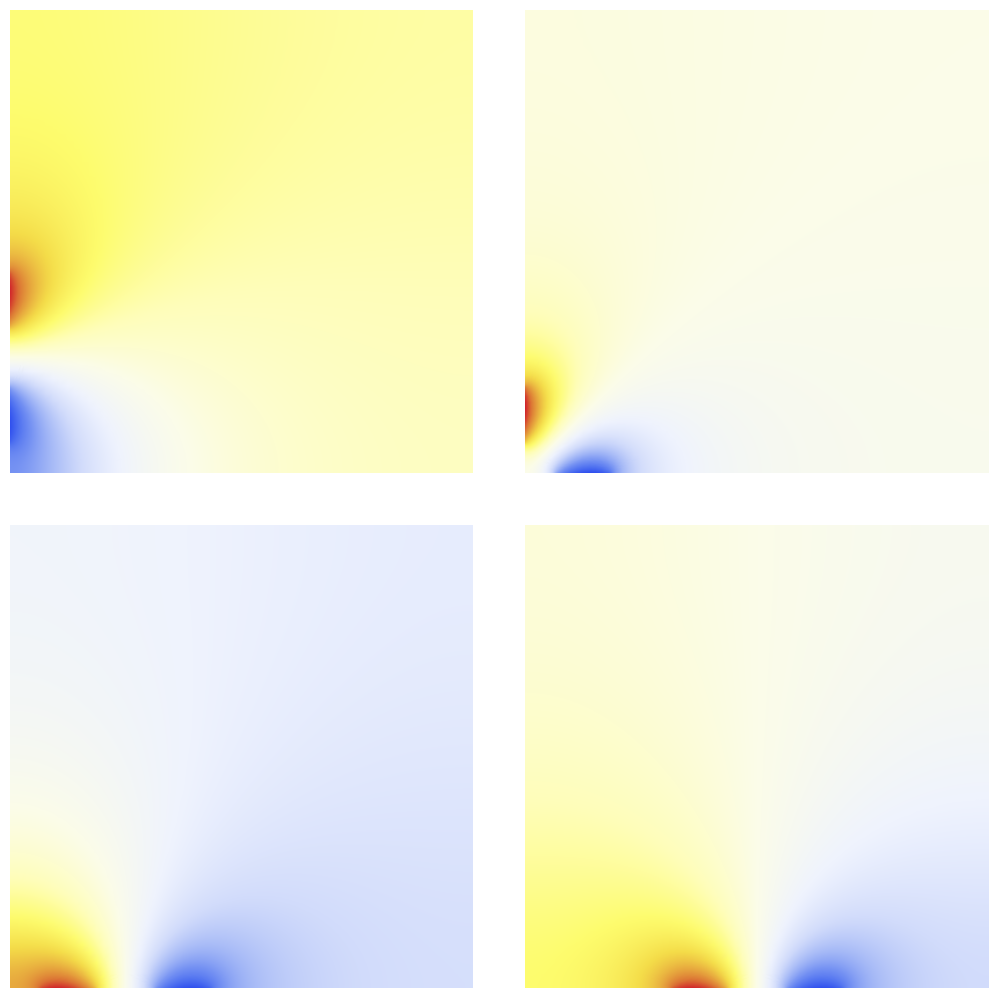
\includegraphics[width=0.16\textwidth]{./hakula/potentials}\qquad
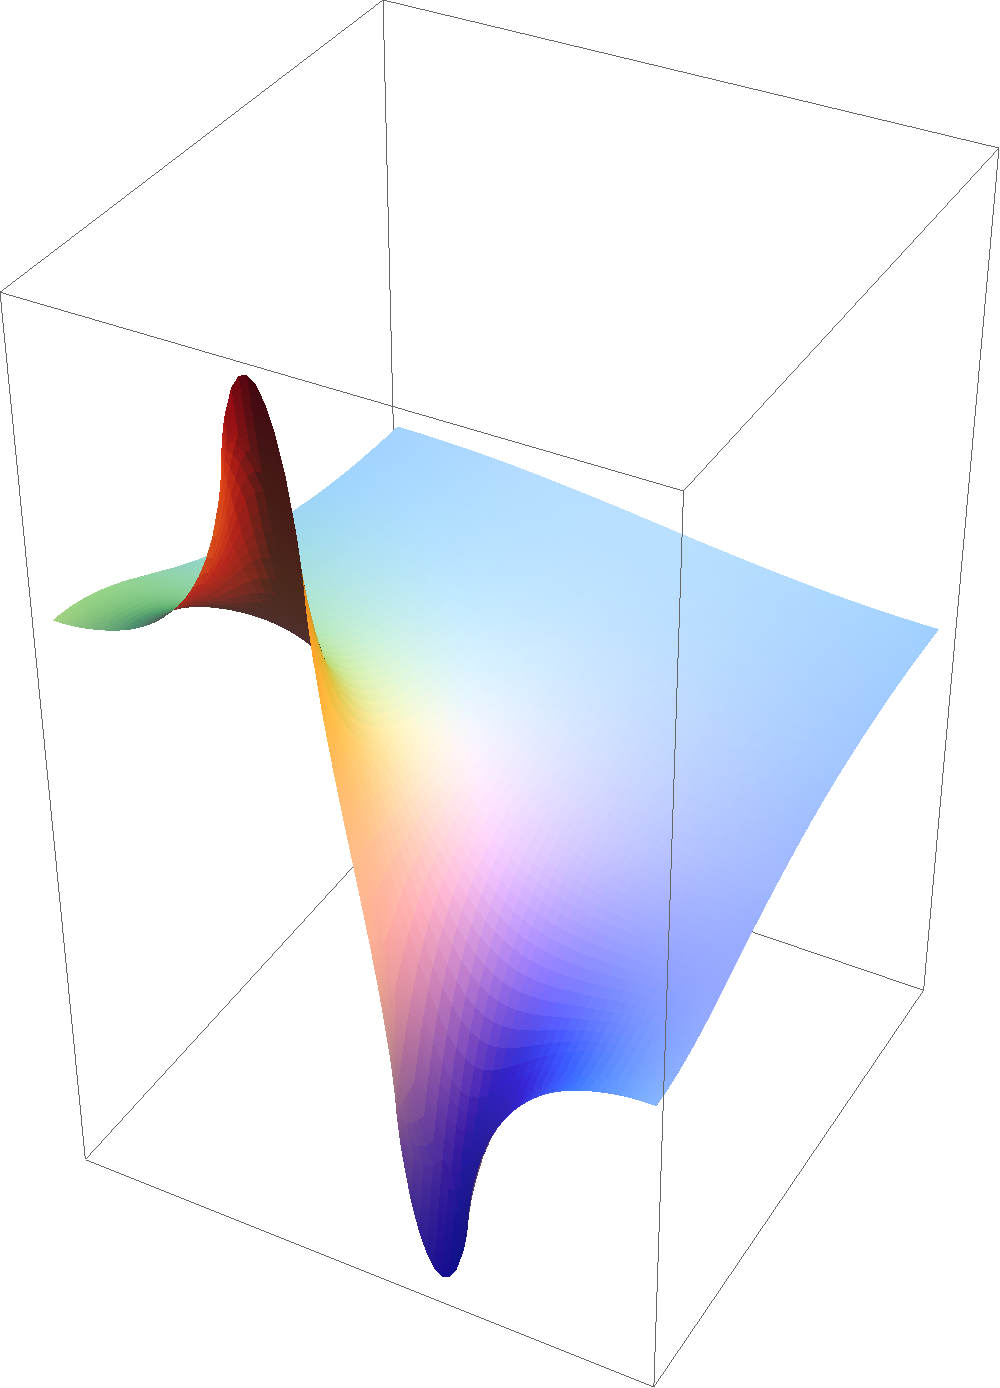
\includegraphics[height=1.25in]{./hakula/potential3d}\qquad
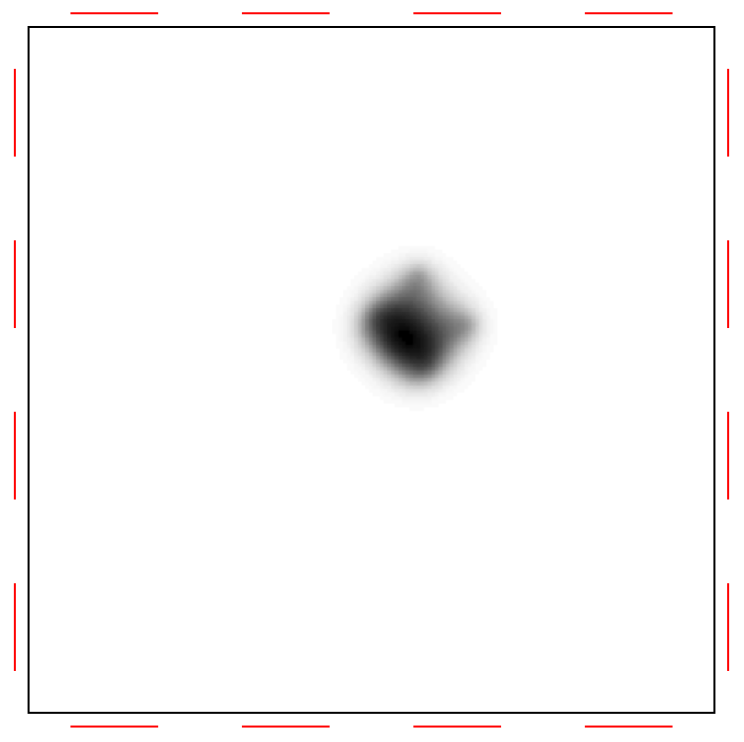
\includegraphics[width=0.15\textwidth]{./hakula/reconstruction}\newline
\caption{Domain with electrodes and inclusion. Electrode pair potentials (2D\&3D). Reconstruction \cite{LHH}.}%
\label{fig}
\end{figure}

\bibliographystyle{plain}
\begin{thebibliography}{10}

\bibitem{LHH} {\sc A.~Lechleiter, N.~Hyvnen, H.~Hakula}, 
{The factorization method applied to the complete electrode model of impedance tomography}. SIAM Journal on Applied Mathematics, 68, pp.~1097--1121 (2008).
\bibitem{HT} {\sc H.~Hakula and T.Tuominen}, IOP Conf. Ser.: Mater. Sci. Eng. 10 012163

\end{thebibliography}